\maketitle
\tableofcontents
\newpage
\section{Theorie}
Ziel des Versuchs ist das Verständnis der Untersuchung von Strömungen mithilfe des
Impuls-Echo-Verfahrens der Ultraschalltechnik. Das Impuls-Echo-Verfahren beruht auf dem akustischen Dopplereffekt,
also der Frequenzveränderung einer Schallwelle bei einer Relativbewegung zwischen Quelle
und Sender. Benutzt wird dabei das als Ultraschall bezeichnete Frequenzband zwischen
\SI{20}{\kilo\hertz} und \SI{1}{\giga\hertz}. Unterschieden wird beim akustischen
Dopplereffekt zwischen zwei Fällen:
\begin{enumerate}
  \item \textbf{Bewegte Quelle - Ruhender Empfänger:}
  Bei Annäherung einer mit Geschwindigkeit $v$ bewegten Quelle misst der Beobachter eine um den
  Faktor $\left(1 - \frac{v}{c} \right)^{-1}$ erhöhte gesendete Frequenz $\nu_0$, bewegt sich
  die Quelle in die andere Richtung, so sinkt $\nu_0$ um den Faktor $\left(1 + \frac{v}{c} \right)^{-1}$.
  Zusammenfassend ist die gemessene Frequenz also durch
  \begin{equation}
    \label{eq:1}
    \nu_{\symup{kl/gr}} = \frac{\nu_0}{1 \mp \frac{v}{c}}
  \end{equation}
  \item \textbf{Bewegter Empfänger - Ruhende Quelle:}
  In diesem Fall bewirkt eine Annäherung eine Verschiebung von $\nu_0$ um den Faktor
  $ \left(1+ \frac{v}{c} \right) $, im umgekehrten Fall tritt eine Verminderung um den
  $ \left(1- \frac{v}{c} \right) $, in einer Formel also:
  \begin{equation}
    \label{eq:2}
    \nu_{\symup{h/n}} = \nu_0 \left( 1 \pm \frac{v}{c} \right)
  \end{equation}
\end{enumerate}
In der Doppler-Sonographie findet nun der zweite Fall Anwendung um beispielsweise
Strömungsgeschwindigkeiten zu bestimmen. Aus \eqref{eq:2} folgt eine Frequenzverschiebung von
\begin{equation}
  \label{eq:3}
  \symup{\Delta}\nu = \nu_0 \frac{v}{c} (\cos{\alpha} + \cos{\beta}),
\end{equation}
die Winkel $\alpha$ und $\beta$  sind dabei die zwischen dem Geschwindigkeitsvektor des
beobachteten Teilchens und dem Normalenvektor der einlaufenden bzw. der am Objekt reflektierten
auslaufenden Wellenfront eingeschlossenen Winkel. Beim Impuls-Echo-Verfahren sind
Sender und Empfänger in einem Gerät zusammengefasst, sodass $\alpha$ und $\beta$ geich sind
und aus \eqref{eq:3}
\begin{equation}
  \label{eq:4}
  \symup{\Delta}\nu = 2 \nu_0 \frac{v}{c} \cos{\alpha}
\end{equation}
folgt. Das Verfahren ist in Abbildung \ref{abb:1} dargestellt.
\begin{figure}
  \centering
  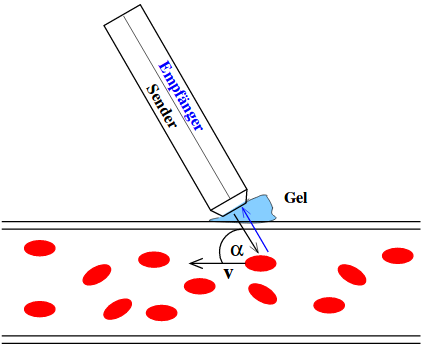
\includegraphics[scale=0.35]{blutbahn.png}
  \caption{Schematische Skizze der Doppler-Sonographie \cite{anleitung}.}
  \label{abb:1}
\end{figure}
Erzeugt werden kann Ultraschall unter Zuhilfenahme des piezo-elektrischen Effekts.
Ein piezoelektrischer Kristall, meist Quartze, wird duch ein sich periodisch änderndes elektrisches Feld
zu Schwingungen angeregt und strahlt dadurch Ultraschallwellen ab. Trifft die Frequenz mit
der das Feld umgepolt wird im Resonanzfall mit der Eigenfrequenz des Kristalls überein,
erreichen die abgestrahlten Ultraschallwellen hohe Amplituden und damit auch hohe Energieichten.
Der piezo-elektrische Effekt an Kristallen kann im umgekehrten Fall als Empfänger
genutzt werden. Einlaufende Schallwellen regen den Kristall dabei zu Schwingungen an.
\section{Durchführung}
\subsection{Versuchsaufbau}
\label{aufbau}
Der Versuchsaufbau besteht aus einem Flüssigkeitskreislauf, in dem eine Zentrifugalpumpe eine Strömung
erzeugt. Die Strömungsgeschwindigkeit lässt sich dabei stufenlos durch Veränderung
der Pumpleistung regeln. In den Kreislauf integriert sind gerade Rohrstücke
mit verschiedenen Durchmessern, auf die ein Dopplerprisma aus Acryl aufgesetzt wird,
dessen Oberseite drei vordefinierte Einstrahlwinkel $\theta$
(\SI{15}{\textdegree}, \SI{30}{\textdegree} und \SI{60}{\textdegree}) bietet (siehe Abbildung \ref{abb:2}).
\begin{figure}
  \centering
  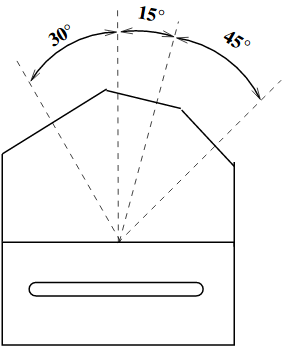
\includegraphics[scale=0.35]{DopplerPrisma.png}
  \caption{Skizze eines Dopplerprismas mit eingezeichneten Einstrahlwinkeln \cite{anleitung}.}
  \label{abb:2}
\end{figure}
Alle Kontaktflächen werden mit einem
Gel eingerieben, um die Übertragung der Ultraschallwellen zu optimieren.
Diesen Einstrahlwinkeln wird mit der Schallgeschwindigkeiten der Flüssigkeit ($c_\symup{L}$) und des Prismas
($c_\symup{P}$) durch das Brechungsgesetz ein Dopplerwinkel
\begin{equation}
  \label{eq:5}
  \alpha = \SI{90}{\textdegree} - \arcsin \left( \sin \theta \cdot \frac{c_\symup{L}}
  {c_\symup{P}} \right)
\end{equation}
zugeordnet. Genutzt wird eine Schallfrequenz $\nu_0$ von \SI{2}{\mega\hertz}. Die Messsonde
ist währenddessen über einen Ultraschall Doppler-Generator mit einem Computer verbunden, auf dem ein
Messprogramm installiert ist, welches das Auslesen der gemessenen Daten ermöglicht. Die
verwendete Flüssigkeit ist bezüglich ihrer akustischen Eigenschaften auf die
verwendeten Frequenz angepasst.
\subsection{Versuchsdurchführung}
In einem ersten Teil wird die Strömungsgeschwindigkeit in einem Rohrstück aus den
verschiedenen Einstrahlwinkeln des Doppler-Prismas bestimmt. Es werden für
fünf verschiedene Pumpeinstellungen aus allen drei Einstrahlwinkeln die Frequenzverschiebung
$\symup{\Delta}\nu$ gemessen. Daraus ergibt sich nach Formel \eqref{eq:4} mit Formel \eqref{eq:5}
die Strömungsgeschwindigkeit. Die jeweiligen Dopplerwinkel $\symup{\Delta}\nu / \cos \alpha$
werden dann in Abhängigkeit der Strömungsgeschwindigkeit in einem Diagramm aufgetragen.\\
\\
In einer zweiten Messreihe wird das Strömungsprofil in einem \num{3/8}-Zoll Rohr
(ca. \SI{10}{\milli\meter}) unter einem Einstrahlwinkel von \SI{15}{\textdegree} bestimmt.
Gemessen wird bei einer Pumpleistung von \SI{45} und \SI{70}{\percent}. Der Ultraschall
Doppler-Generator wird so eingestellt, dass er einer variable Messtiefe liefert.
Die Einstellung am Generator ist dabei in \SI{0.5}{\micro\second}-Schritten möglich,
die Umrechnung in \si{\milli\metre} ist materialabhängig. Es wird der komplette
Rohrduchmesser durchfahren und in \SI{0.75}{\milli\metre}-Abständen sowohl Strömungsgeschwindigkeit als
auch Streuintensitätswert gemessen. Die beiden Datenreihen werden in Abhängigkeit der
Messtiefe in einem Diagramm aufgetragen.
\section{Auswertung}
Die im folgenden ausgewerteten Versuchsteile wurden an einem Rohr mit einem Durchmesser
von $\SI{0.01}{\meter}$ durchgeführt.
\subsection{Bestimmung der Strömungsgeschwindigkeit für die Dopplerwinkel.}
Um die Strömungsgeschwindigkeit zu bestimmmen, wird \eqref{eq:4}
umgeformt zu
\begin{equation}
    v = \frac{\symup{\Delta} \nu \cdot c}{2 \, \nu_0 \, \symup{cos} \, \alpha} \, .
    \label{eqn:6}
\end{equation}
Mit \eqref{eq:5} folgt für die Dopplerwinkel $\alpha$ aus \eqref{eqn:6}
\begin{table}
  \centering
  \begin{tabular}{c c}
    \toprule
    $\theta$ & $\alpha$ \\
    \midrule
    15° & 80.06° \\
    30° & 70.53° \\
    60° & 54.74° \\
    \bottomrule
  \end{tabular}
  \caption{Dopplerwinkel $\alpha$ zu den vordefinierten Einfallswinkeln $\theta$.}
  \label{tab:1}
\end{table}
mit $c_L = \SI{1800}{\meter\per\second}$ und $c_P = \SI{2700}{\meter\per\second}$.
Damit folgen die Ergebnisse für die drei Dopplerwinkel mit $\nu_0 = \SI{2}{\mega\hertz}$
und $c = \SI{1800}{\meter\per\second}$ mit dem jeweils passendem Diagramm.
\begin{figure}
  \begin{subfigure}{0.6\textwidth}
    \centering
      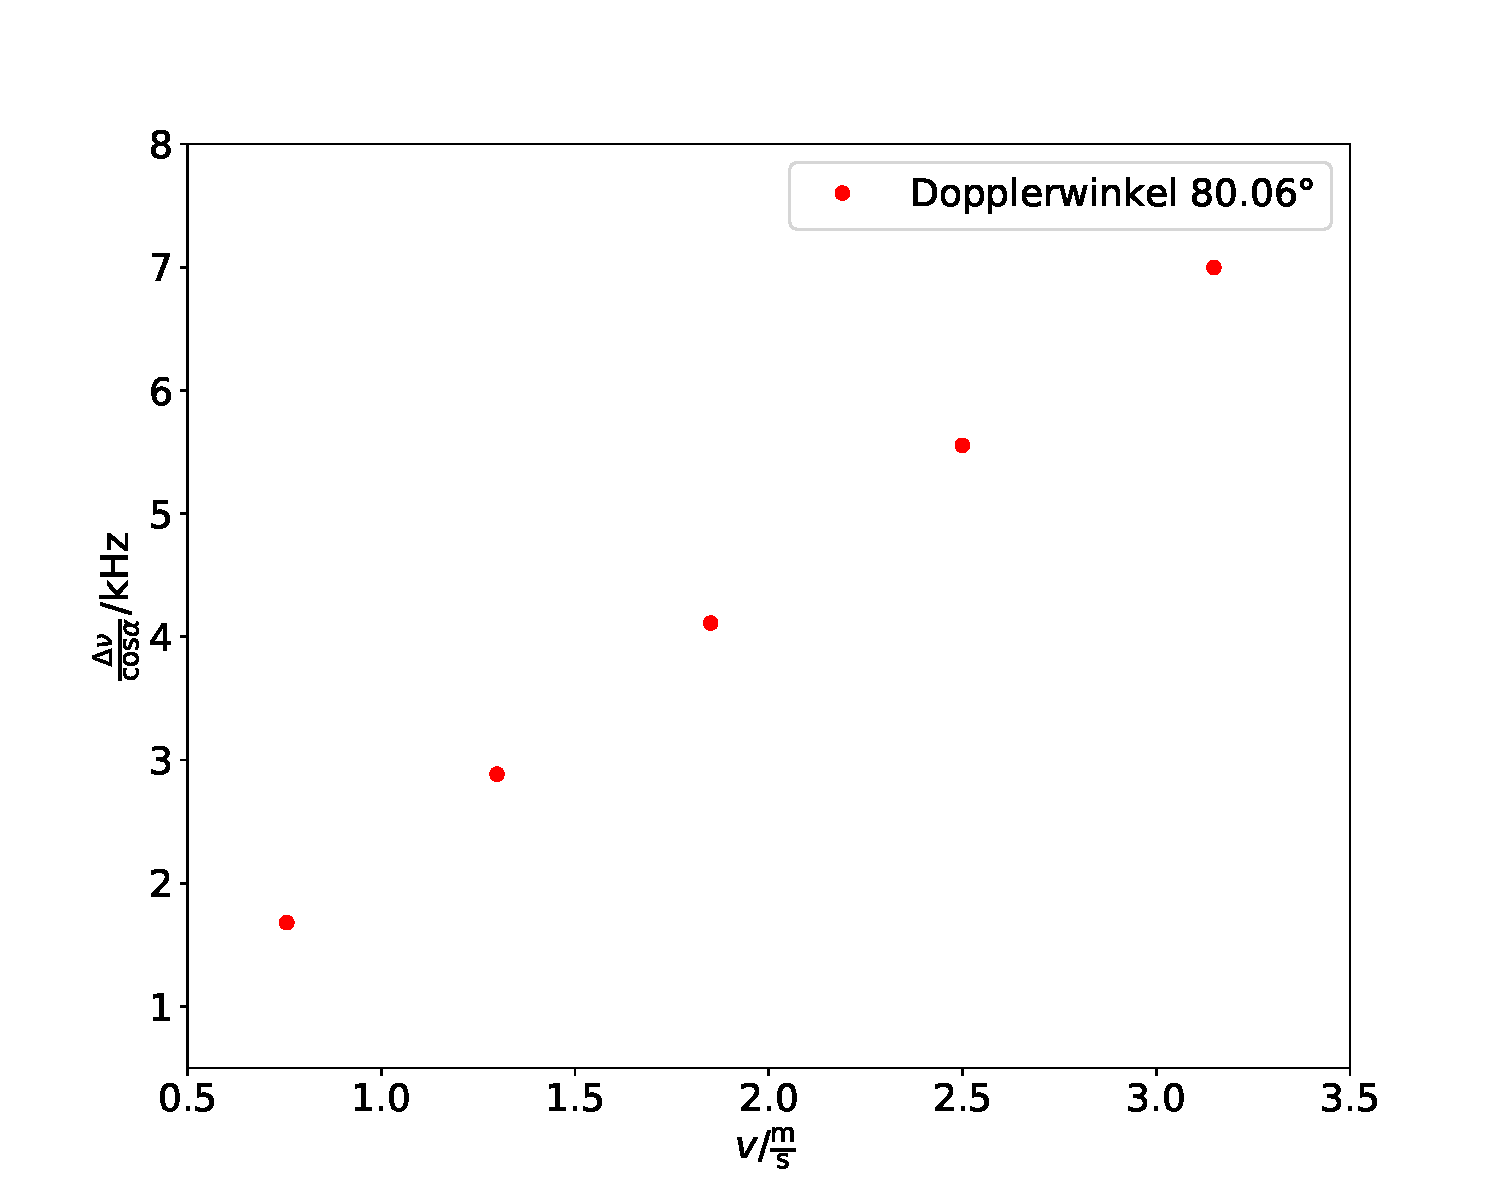
\includegraphics[width=\textwidth]{a15.pdf}
      \caption{Diagramm für 15°.}
      \label{fig:1}
      \qquad
  \end{subfigure}
  \begin{subtable}{0.4\textwidth}
    \centering
    \begin{tabular}{c c c}
      \toprule
      Pumpleistung / $\%$ & $\symup{\Delta} \nu$ / $\si{\hertz}$ & $v$ / \si{\meter\per\second} \\
      \midrule
      30 & -85 & 0.76 \\
      40 & -146 & 1.30 \\
      50 & -208 & 1.85 \\
      60 & -281 & 2.50 \\
      70 & -354 & 3.15 \\
      \bottomrule
    \end{tabular}
    \caption{Strömungsergebnisse für 15°.}
    \label{tab:2}
    \qquad
  \end{subtable}
  \caption{Ergebnisse für den Dopplerwinkel 80.06°.}
\end{figure}

  \begin{figure}
      \begin{subfigure}{0.6\textwidth}
      \centering
        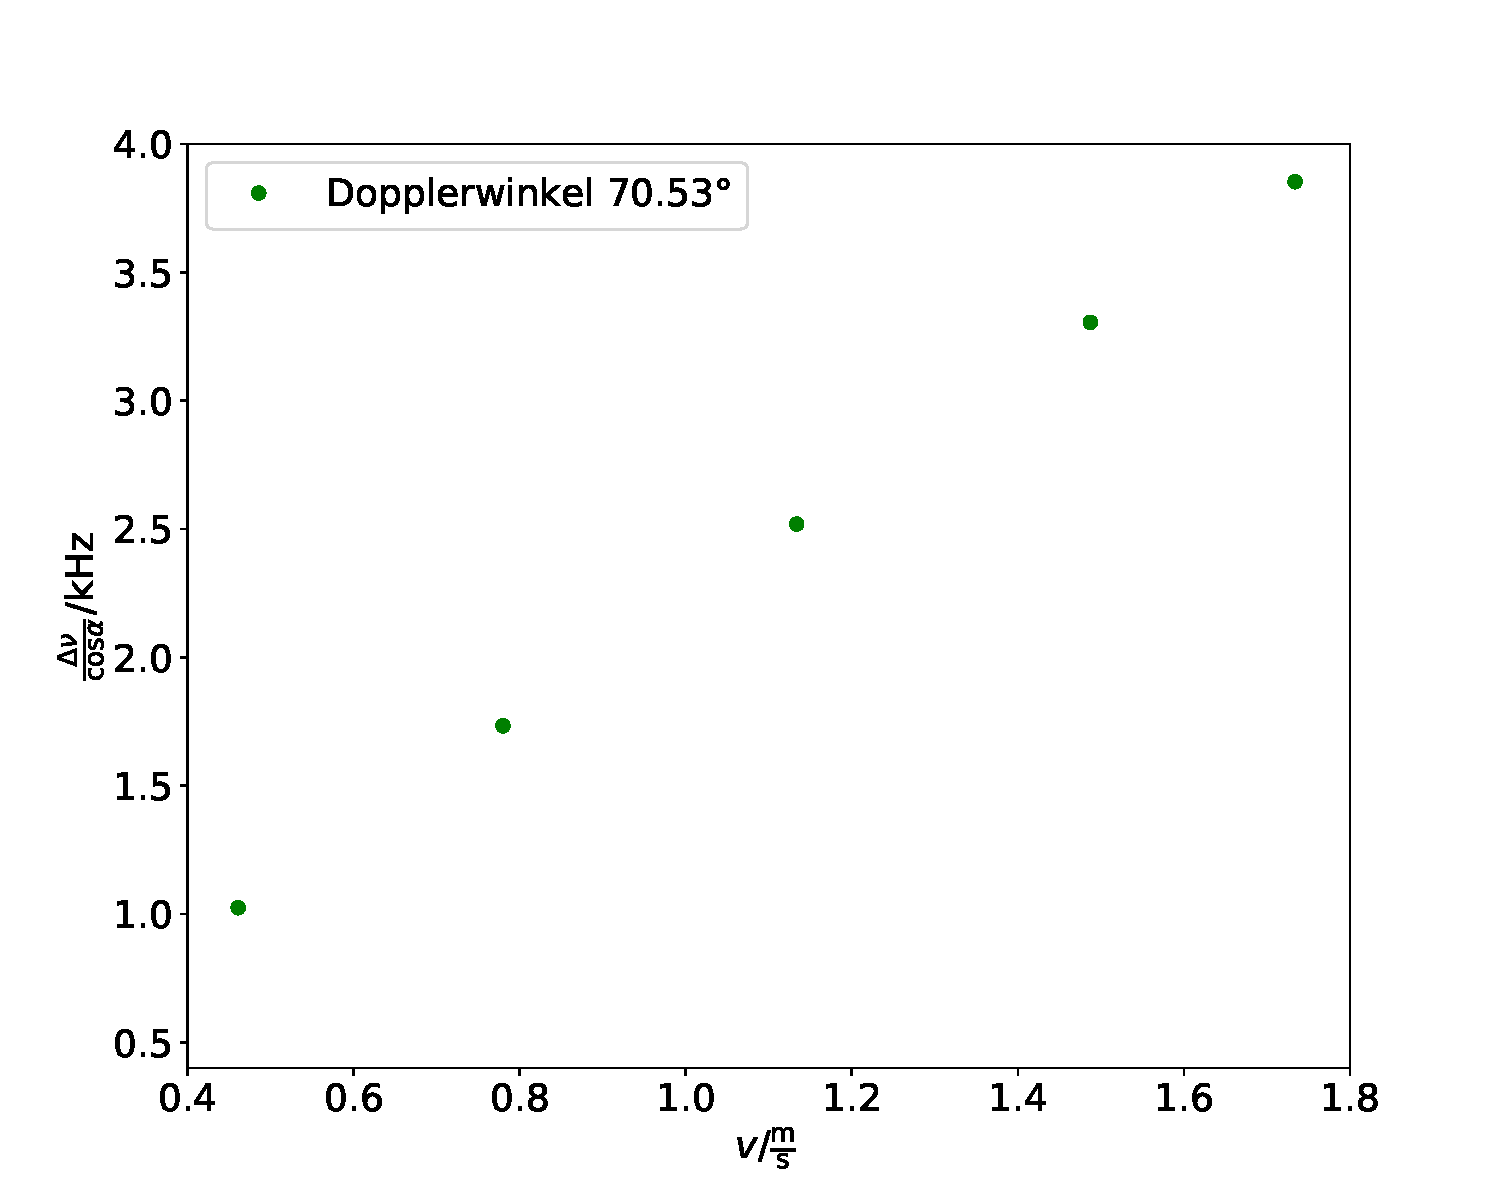
\includegraphics[width=\textwidth]{a30.pdf}
        \caption{Diagramm für 30°.}
        \label{fig:2}
        \qquad
    \end{subfigure}
    \begin{subtable}{0.4\textwidth}
      \centering
      \begin{tabular}{c c c}
        \toprule
        Pumpleistung / $\%$ & $\symup{\Delta} \nu$ / $\si{\hertz}$ & $v$ / \si{\meter\per\second} \\
        \midrule
        30 & 159 &  0.46100395\\
        40 & 269 &  0.7799375 \\
        50 & 391 & 1.1336638  \\
        60 & 513 & 1.4873901  \\
        70 & 598 & 1.73383875 \\
        \bottomrule
      \end{tabular}
      \caption{Strömungsergebnisse für 30°.}
      \label{tab:3}
      \qquad
    \end{subtable}
    \caption{Ergebnisse für den Dopplerwinkel 70.53°.}
  \end{figure}
    \begin{figure}
      \begin{subfigure}{0.6\textwidth}
        \centering
          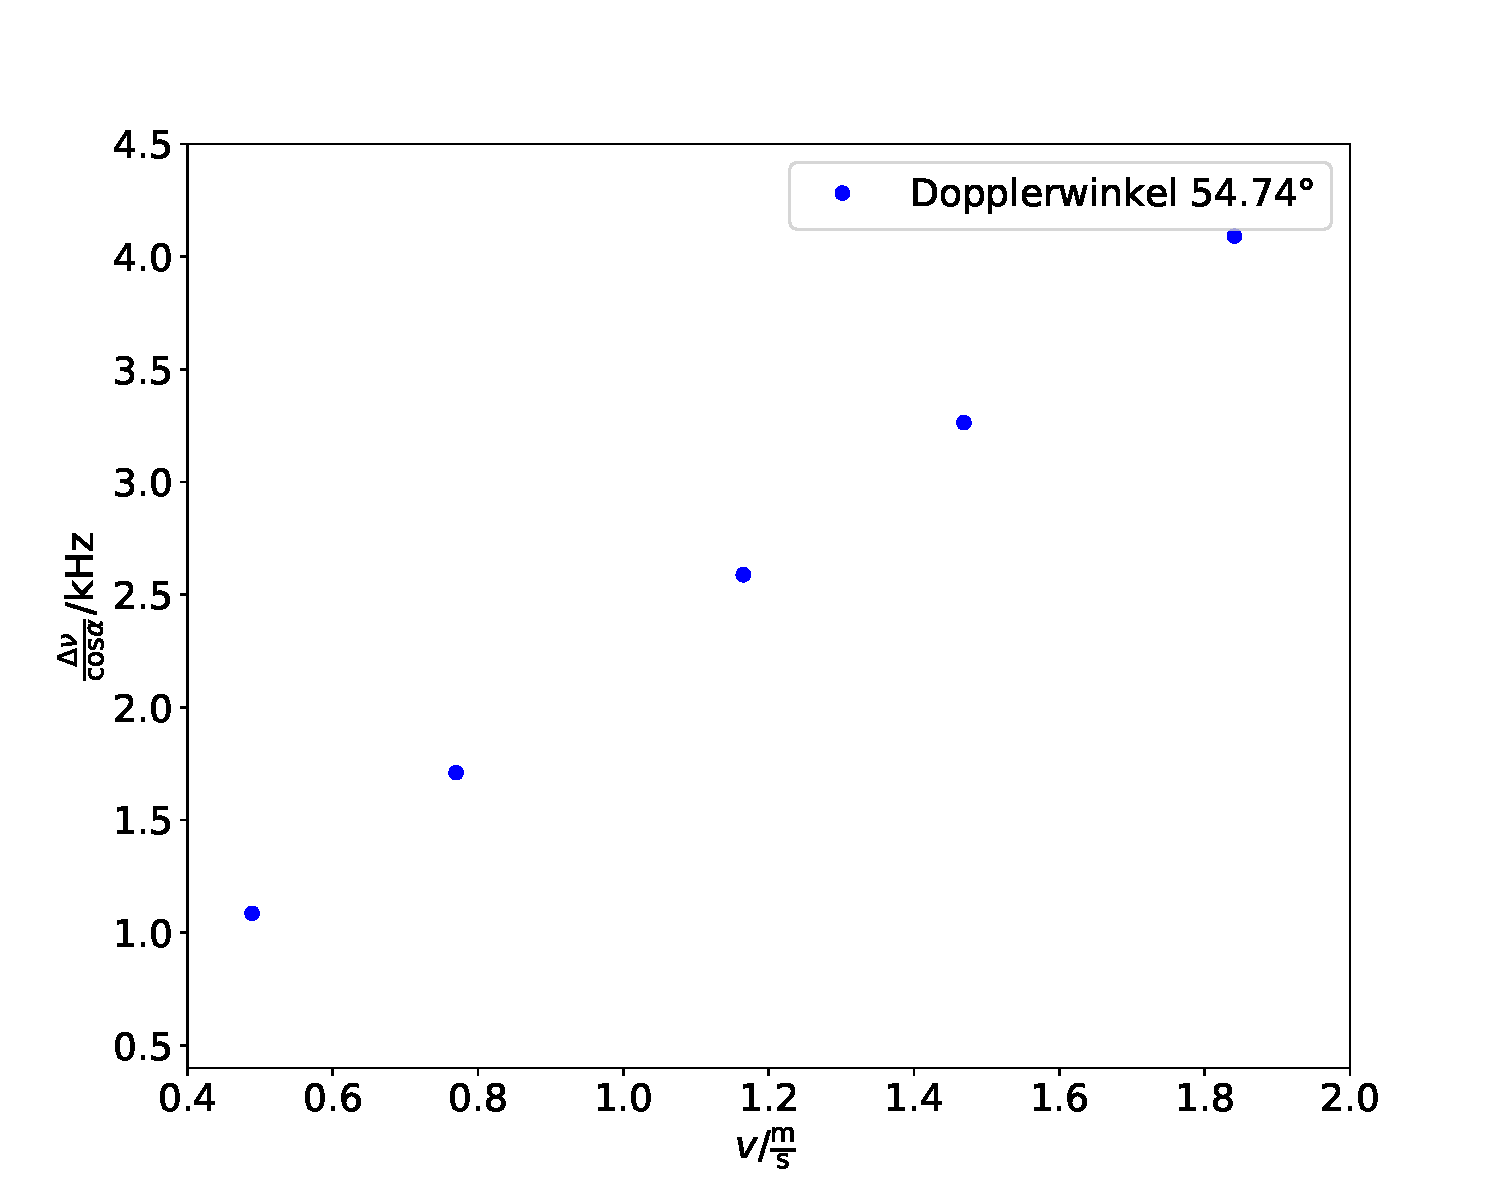
\includegraphics[width=\textwidth]{a60.pdf}
          \caption{Diagramm für 60°.}
          \label{fig:3}
          \qquad
      \end{subfigure}
      \begin{subtable}{0.4\textwidth}
        \centering
        \begin{tabular}{c c c}
          \toprule
          Pumpleistung / $\%$ & $\symup{\Delta} \nu$ / $\si{\hertz}$ & $v$ / \si{\meter\per\second} \\
          \midrule
          30 & -256 & 0.49 \\
          40 & -403 & 0.77 \\
          50 & -610 & 1.16 \\
          60 & -769 & 1.47 \\
          70 & -964 & 1.84 \\
          \bottomrule
        \end{tabular}
        \caption{Strömungsergebnisse für 60°.}
        \label{tab:4}
        \qquad
      \end{subtable}
      \caption{Ergebisse für den Dopplerwinkel 54.74°.}
    \end{figure}
      \subsection{Bestimmung der Streuintensität und der Momentangeschwindigkeit in
      Abhängigkeit von der Messtiefe}
      Zur Bestimmung der Momentangeschwindigkeit wird \eqref{eqn:6} genutzt mit
      $\alpha = 80.06°$ und dem gemessenen Wert für $\symup{\Delta} \nu$. Für $\nu_0$
      wird $\SI{2}{\mega\hertz}$ (vgl. Kapitel \ref{aufbau}) und für c
      $\SI{1800}{\meter\per\second}$ verwendet.
      \begin{figure}
        \centering
        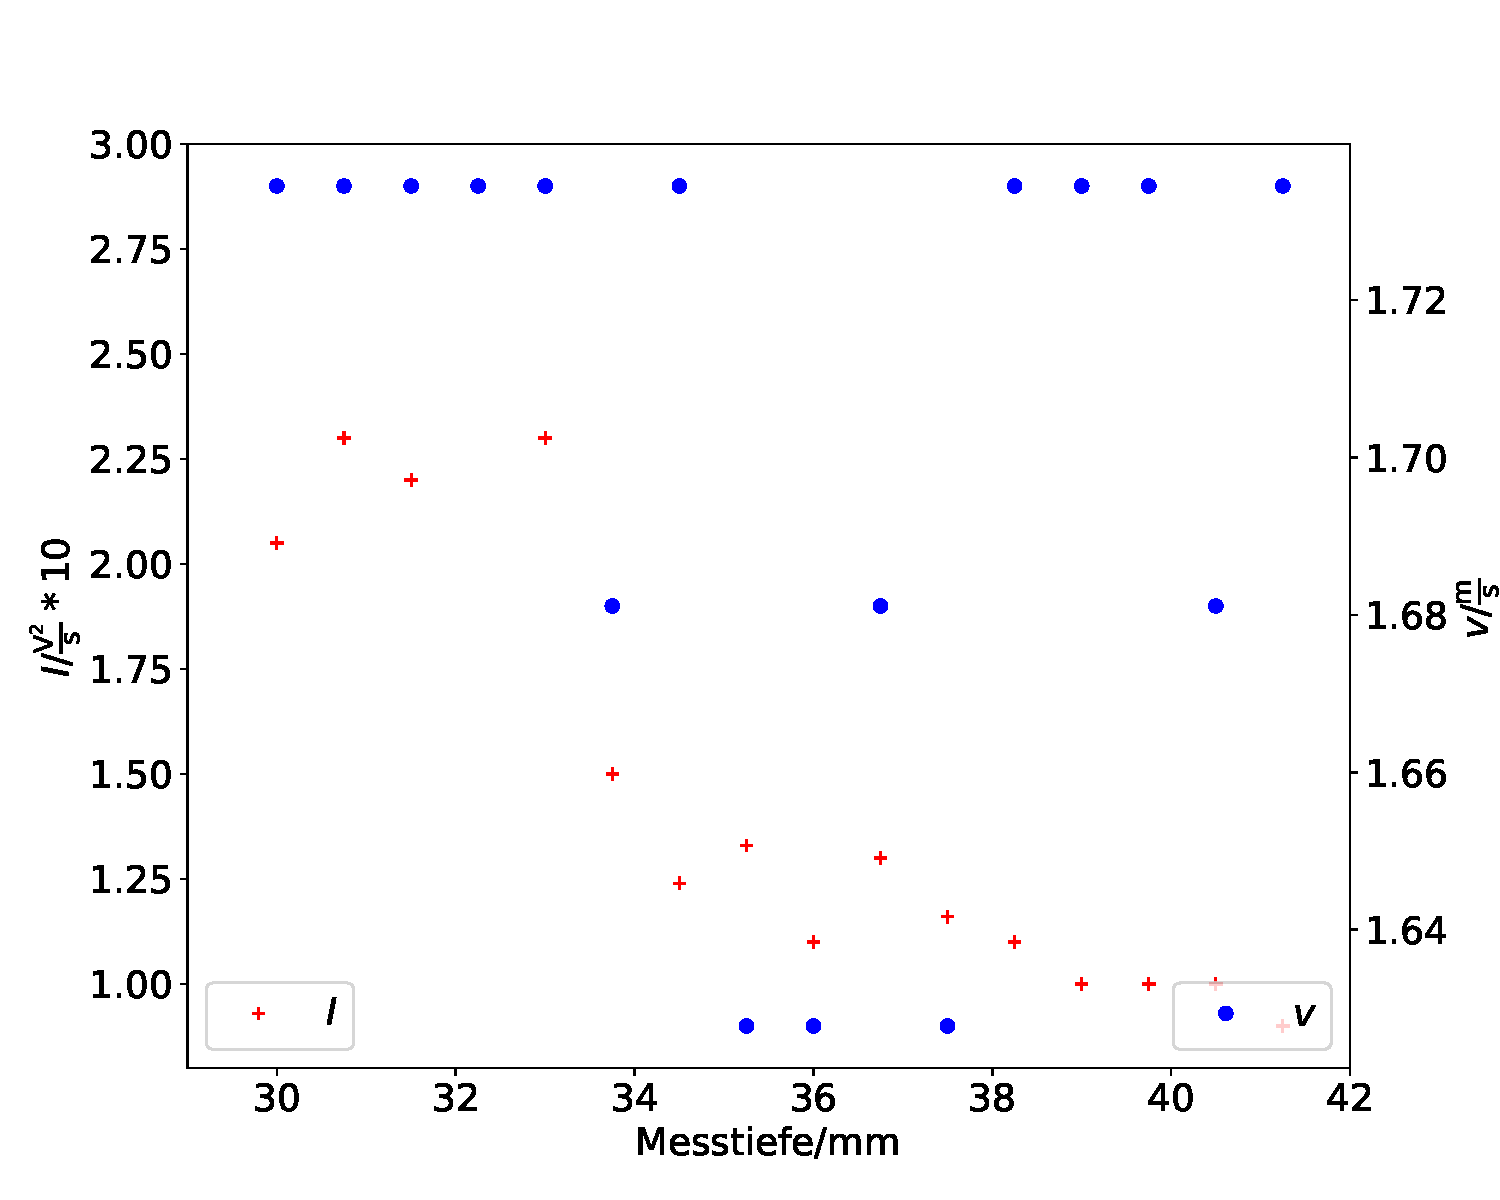
\includegraphics[scale=0.3]{b45.pdf}
        \caption{Momentangeschwindigkeit und Streuintensität in Abhängigkeit von der Messtiefe
        bei 45$\%$ Pumpleistung.}
        \label{fig:4}
      \end{figure}
      \begin{figure}
        \centering
        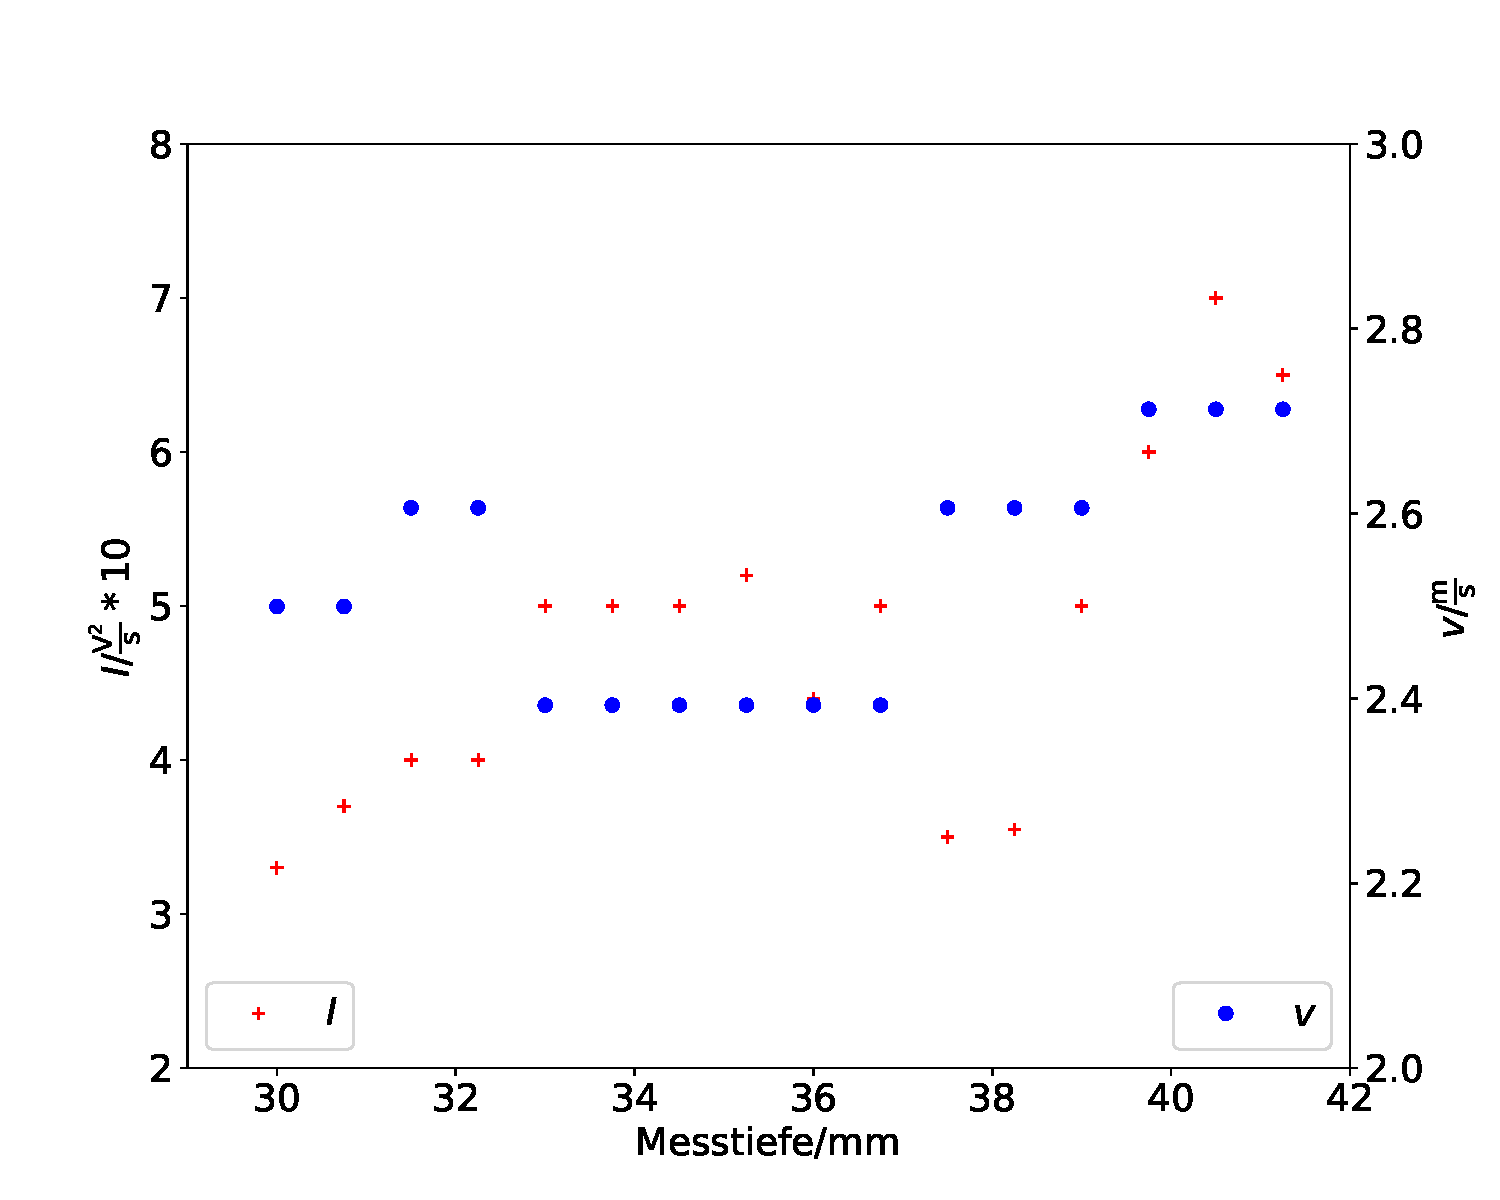
\includegraphics[scale=0.3]{b70.pdf}
        \caption{Momentangeschwindigkeit und Streuintensität in Abhängigkeit von der Messtiefe
        bei 70$\%$ Pumpleistung.}
        \label{fig:5}
      \end{figure}
\section{Diskussion}
\newpage
\nocite{*}
\printbibliography
